\section{Algorithm and Implementation}\label{sec:model}


\begin{figure}[tb]
	\centering
	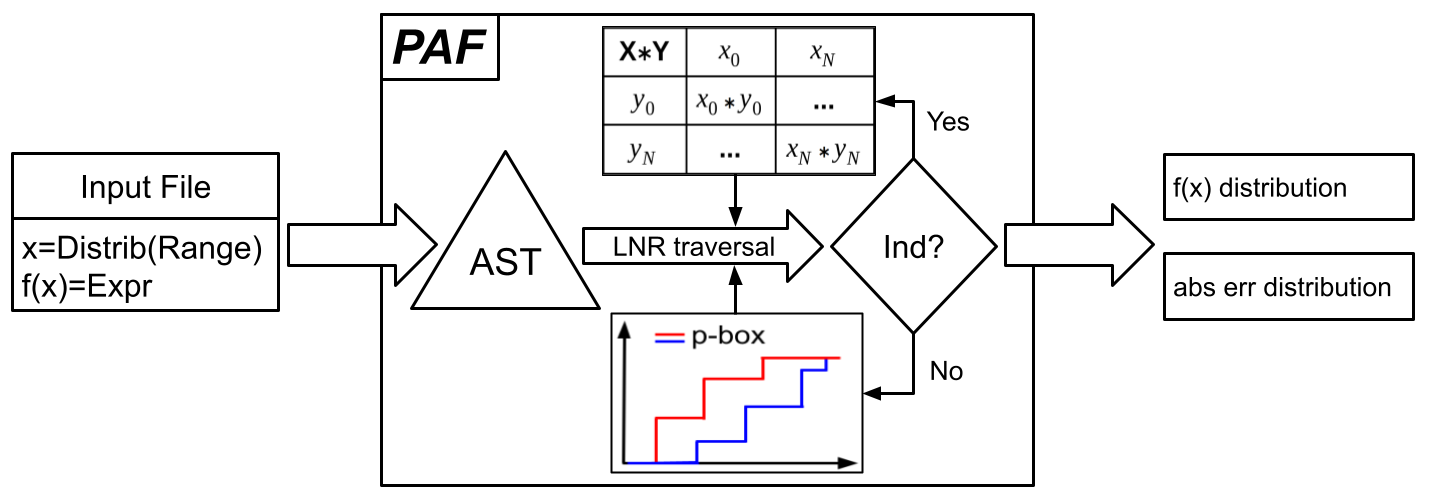
\includegraphics[width=\textwidth]{pics/toolflow.png}
	\caption{Toolflow of \Tool.}
	\label{fig:toolflow}
\end{figure}


In this section, we describe our probabilistic model of floating-point
arithmetic and how we implement it in a prototype named \Tool (for
Probabilistic Analysis of Floating-point errors).
%
Fig.~\ref{fig:toolflow} shows the toolflow of \Tool.
%

%In \cref{subsec:inputlanguage}, we show the input language of \Tool and how we
%interpret operands and operations.
%
%Then in \cref{subsec:probmodel}, we describe the probabilistic model of
%floating-point arithmetic used in \Tool, and what are the routines \Tool runs
%in case of independent (\cref{subsec:modelAnalysis}) and dependent
%(\cref{subsec:dependentOperation}) operations.
%
%Finally, we report the procedure used in \Tool to compute the bounds for the
%roundoff errors in~\cref{subsec:conderror}.
%

%\subsection{Input Language}\label{subsec:inputlanguage}

\subsection{Probabilistic model}\label{subsec:model}
\Tool takes as input a text file describing a probabilistic floating-point
computation and its input distributions.
%
The kinds of computations we support are captured with this simple grammar:
\[
\tt t::= z \mid x_i \mid t\mop t \qquad \mathtt{z}\in\F, \mathtt{i}\in\N, \mop\in\{+,-,\times,\div\}
\]
Following ~\cite{K81c}, we interpret each computation $\tt  t$ given by the grammar as a random variable.
%
We define the interpretation map $\sem{-}$ over the computation tree inductively.
%
The base case is given by
$\sem{\mathtt{z}(s,e,k)} \defeq (-1)^s2^e(1+k2^{-p})$ and $\sem{\mathtt{x_i}} \defeq X_i$,
where the real numbers $\sem{\mathtt{z}(s,e,k)}$ are understood as constant random variables and each $X_i$ is a random input variable
with a user-specified distribution.
%
Currently, \Tool supports several well-known distributions out-of-the-box (e.g., uniform, normal, exponential, beta), and a user can also define custom distributions as piecewise functions.
%
For the inductive case $\sem{\tt t_1\mop t_2}$, we put the lessons from \cref{sec:errordist} to work.
Recall first the probabilistic model \cref{eq:probabilistic}:
\[
x\mop y=(x\iop y)(1+\delta), \qquad\delta\sim dist
\]
%
%
In \cref{subsec:LPerror_dist}, we showed that $dist$ should be taken as the distribution of the actual roundoff errors of the random elements $(x\iop y)$.  We therefore define:
\begin{align}
\sem{\mathtt{t_1 \mop t_2}}\defeq(\sem{\mathtt{t_1}}\iop\sem{\mathtt{t_2}})\times (1+ \erel(\mathtt{\sem{t_1}\iop\sem{\tt t_2})}).\label{eq:model}
\end{align}
To evaluate the model of \cref{eq:model}, we first use the appropriate closed-form expression \cref{eq:LPerrorDensity,eq:HPerrorDensity,eq:typicalpdf}  derived in \cref{sec:errordist} to evaluate the (distribution of the) random variable $\erel(\mathtt{\sem{t_1}\iop\sem{\tt t_2})}$ --- or the corresponding p-box as described in \cref{subsec:errorpbox}. We then use \cref{thm:covar} to justify evaluating the multiplication operation in \cref{eq:model} \emph{independently} --- that is to say by using \cref{eq:pdfarithm} --- since the roundoff process is very close to being uncorrelated to the process generating it. The validity of this assumption is also confirmed experimentally by the remarkable agreement of Monte-Carlo simulations with this analytical model (see \cref{sec:evaluation}).


%\subsection{Evaluating Arithmetic Expressions over Random Variables}\label{subsec:modelAnalysis}
%With the model of \cref{eq:model} and its evaluation strategy in place,  it now remains to evaluate arithmetic operations between random variable such as $(\sem{\tt t_1}\iop\sem{\tt t_2})$ in infinite precision. As mentioned in the introduction and in \ref{subsec:prob} this is straightforward if the two random variables are independent (we then simply use \cref{eq:pdfarithm}, but it is much harder when the random variables are dependent.
%
We now introduce the algorithm for evaluating the model given in \cref{eq:model}.
%
The evaluation performs an in-order (LNR) traversal of the \emph{Abstract
Syntax Tree} (AST) of a computation given by our grammar, and it feeds the
results to the parent level along the way.
%
At each node, it computes the probabilistic range of the intermediate result
using the probabilistic ranges computed for its children nodes (i.e.,
operands).
%
We first determine whether the operands are independent or not (Ind?\ branch in the toolflow),
and we either apply a cheaper (i.e., no SMT solver invocations) algorithm if they are independent (see below) or
a more involved one (see \cref{subsec:dependentOperation}) if they are not.
%
We describe our methodology at a generic intermediate computation in the AST of the expression. 


We consider two distributions $X$ and $Y$ discretized into DS-structures $DS_{X}$ and $DS_{Y}$ (\cref{subsec:prob}), and we want to derive the DS-structure $DS_Z$ for $Z=X\iop Y$,  $\iop \in \{+,-,\times,\div\}$.\todo[inline]{Fred: should we say how it's done at the leaves?}
%
Together with the DS-structures of the operands, we also need the traces $trace_X$ and $trace_Y$ containing the history of the operations performed so far, one for each operand. A trace is constructed at each leaf of the AST with the input distributions and their range. It is then propagated to the parent level and populated at each node with the current operation. 
%
Such history traces are critical when dealing with dependent operations since they allow us to interrogate an SMT solver about the feasibility of the current operation, as we describe in the next section.
%
When the operands are independent, we simply use the arithmetic operations on independent DS-structures~\cite{bouissou2012generalization}
(see \cref{sec:appdx-independent}).


\subsection{Computing Probabilistic Ranges for Dependent Operands}\label{subsec:dependentOperation}
%
When the operands are dependent, we start by assuming that the dependency is unknown.
%(as also done by Bouissou et al.~\cite{bouissou2012generalization}).
%
This assumption is sound because the dependency of the operation is included in the set of unknown dependencies, while the result of the operation is no longer a single distribution but a p-box.
%
Due to this ``unknown assumption'', the CDFs of the output p-box are a very pessimistic over-approximation of the operation, i.e., they are far from each other.
%
%The soundness comes with a high cost in terms of accuracy and produces a very pessimistic over-approximation. 
%
Our key insight is to then leverage an SMT solver to prune infeasible combinations of intervals from the input DS-structures, which prunes regions of zero probability from the output p-box.
%
%We use an SMT solver to detect sections of the p-box where the probability is zero. 
%
%In other words, thanks to the solver, we can identify infeasible regions in the p-box and conclude the probability there is zero.
%
This probabilistic pruning using a solver squeezes together the CDFs of the output p-box, often resulting in a much more accurate over-approximation.
%
Thanks to using a solver, we move from an unknown to a \emph{partially known} dependency between the operands.
%
Currently, \Tool supports the Z3~\cite{Z3} and dReal~\cite{dReal} SMT solvers.


\begin{algorithm}[tb]
	\caption{Dependent Operation $Z=X\iop Y$}\label{dependentalg}
	\begin{algorithmic}[1]
		\Function {dep\_op}{$DS_X,\iop,DS_Y,trace_X,trace_Y$}
		\State $DS_Z=list()$
		\ForAll {$ ([x_1, x_2], p_{x}) \in DS_X$} 
		\ForAll {$ ([y_1, y_2], p_{y}) \in DS_Y$}
		\State $[z_1, z_2]=[x_1, x_2] \iop\;[y_1, y_2]$ \Comment{operation between intervals}
		\State $[z_1', z_2']=SMT.prune([z_1, z_2])$
		\If {$SMT.check(trace_X \land trace_Y \land [x_1, x_2] \land [y_1, y_2])$ \textbf{is} $SAT$}
		\State $p_Z=\mbox{unknown-probability}$
		\Else 
		\State $p_Z=0$
		\EndIf
		\State $DS_Z.append(([z_1', z_2'],p_Z))$
		\EndFor
		\EndFor
		\State $trace_Z=trace_X \cup trace_Y\cup\{Z=X\iop Y\}$
		\State \textbf{return} $DS_Z, trace_Z$
		\EndFunction
	\end{algorithmic}
\end{algorithm}


\cref{dependentalg} shows the pseudocode of our algorithm for computing the
probabilistic output range (i.e., DS-structure) for dependent operands.
%
When dealing with dependent operands, interval arithmetic (line 5) might not be as precise as in the independent case.
%
Hence, we use an SMT solver to prune away any over-approximations introduced by
interval arithmetic when computing with dependent ranges (line 6);
this use of the solver is orthogonal to the one dealing with probabilities.
%
On line 7, we check with an SMT solver whether the current combination of
ranges $[x_1, x_2]$ and $[y_1, y_2]$ is compatible with the traces of the
operands.
%
If the query is satisfiable, the probability is strictly greater than zero but currently unknown (line 8).
%
If the query is unsatisfiable, we assign a probability of zero to the range in $DS_Z$ (line 10). 
%
%The immediate consequence of pruning is the p-box is going to squeeze around the output distribution.
%
%Clearly, the SMT solver allows us to handle also non-linear dependencies between the operands.
%
%
Finally, we append a new range to the DS-structure $DS_Z$ (line 11).
%
Note that the loops are independent, and hence in our prototype implementation we run them in parallel.


After this algorithm terminates, we still need to assign probability values to
all the unknown-probability ranges in $DS_Z$.
%
Since we cannot assign an exact value, we compute a range of potential values
$[p_{z_{min}}, p_{z_{max}}]$ instead. 
%
This computation can be encoded as a \emph{linear programming} routine exactly
as described in previous work~\cite{bouissou2012generalization} (see \cref{sec:appdx-lp}).

%We can create a linear programming (LP) routine to delineate upper bound and lower bounds for the p-box.

%\begin{align*}
%1\leq i,j\leq N \land 
%&\text{\textbf{maximize}}\sum_{evp\:\in\:z_{i,j}} p_{z_{i,j}}\\
%&\text{\textbf{subject to}}\quad 0\leq p_{z_{i,j}}\leq 1\\
%&\qquad\qquad\quad\quad \forall i \in [1,N], \sum_{1\leq j\leq N} p_{z_{i,j}} = p_{y_{i}} \\
%&\qquad\qquad\quad\quad \forall j \in [1,N], \sum_{1\leq i\leq N} p_{z_{i,j}} = p_{x_{i}}\\
%\end{align*}
%
%We report the pseudo-code of maximization program for the upper bound in ?.

%
%The probabilities in the DS structures of the operands ($p_{y_i}$, $p_{x_i}$) are called the \emph{marginals}. The focal elements we used to populate $DS_Z$ are called the \emph{insiders} ($p_{z_{i,j}}$).
%
%The constraints in the LP program force the insiders to have a probability between 0 and 1, and they relate the insiders with the marginals. The insiders have to sum up to the marginals. This is very similar to a so called \emph{joint table}.
%

%The LP program takes in input an \emph{evaluation point} (evp) and returns a probability value.
%
%In order to construct the $DS_Z$ exactly we should pick one evaluation point per focal element. This has quadratic complexity.
%
%A good trade-off between accuracy and execution time consists in picking only $N$ out of the $N^2$ evaluation points (e.g. using some heuristics), at the price of a slightly over-approximation.
%
%We run the linear programming routines in parallel, because the analysis of a single evaluation point is completely independent from the others.
%

\subsection{Computing Conditional Roundoff Error}\label{subsec:conderror}

The final step of our toolflow computes the conditional roundoff error by
combining the symbolic affine arithmetic error form of the computation (see
\cref{sec:symbolicaffine}) with the probabilistic range analysis described
above.
%
The symbolic error form gets maximized conditioned on the results of all the
intermediate operations landing in the given confidence interval (e.g., 99\%)
of their respective ranges (computed as described in the previous section).
%
%Note that conditioning only on the last operation of the computation tree
%(i.e., the AST root) would lead to extremely pessimistic over-approximation
%since numerous infeasible intermediate results would not get pruned away.
%
Note that conditioning only on the last operation of the computation tree (i.e., the AST root) would lead to extremely pessimistic over-approximation since all the outliers in the intermediate operations would be part of the maximization routine.
%As we discussed in \cref{subsec:trackingerrors}, the final roundoff error is the result of all intermediate computations. These can amplify or reduce (e.g. cancellation) the magnitude of the final error.
%
This would lead to our tool \Tool computing pessimistic error bounds typical of
worst-case analyzers.
%


\begin{algorithm}[tb]
	\caption{Conditional Roundoff Error Computation}\label{conderror}
	\begin{algorithmic}[1]
		
		\Function {cond\_err}{$DSS, errorForm, confidence$}
		\State {$allRanges=list()$}
		\ForAll {$DS_i \in DSS$}
		\State {$focals=sorted(DS_i,\:key=prob,\: order=descending)$}
		\State {$accumulator=0$}
		\State {$ranges=\text{\O}$}
		\ForAll {$ ([x_1, x_2], p_{x}) \in focals$}
			\State {$accumulator=accumulator+p_{x}$}
			\State {$ranges=ranges \cup [x_1, x_2]$}
			\If {$accumulator \ge confidence$}
				\State $allRanges.append(ranges)$
				\State $\mathbf{break}$
			\EndIf
		\EndFor
		\EndFor
		\State $error=maximize(errorForm, allRanges)$
		\State \textbf{return} $error$
		\EndFunction
	\end{algorithmic}
\end{algorithm}


\cref{conderror} shows the pseudocode of the roundoff error computation
algorithm.
%
The algorithm takes as input a list $DSS$ of DS-structures (one for each
intermediate result range in the computation), the generated symbolic error
form, and a confidence interval.
%
It iterates over all the intermediate DS-structures (line 3), and for each it
determines the ranges needed to support the chosen confidence intervals (lines
4--12).
%
In each iteration, it first sorts the list of range-probability pairs (i.e.,
focal elements) of the current DS-structure by their probability value in a
descending order (line 4).
%
This is a heuristic that prioritizes the focal elements with most of the
probability mass (aka \emph{typicals}) to avoid including the unlikely outliers
(with low probability) that cause large roundoff errors into the final roundoff
error computation.
%
With the help of an accumulator (line 8), we keep collecting focal elements
(line 9) until the accumulated probability satisfies the confidence interval
(line 10).
%
Finally, we maximize the error form conditioned to the collected ranges of all
intermediate operations (line 13).
%
In \Tool, the maximization is done using the rigorous global optimizer
Gelpia~\cite{gelpia}.



%\begin{itemize}
%	\item \texttt{Global variables}:
%	\begin{itemize}
%		\item $N$: fixes the size of all partitions
%	\end{itemize}
%	\item \texttt{Inputs:} 
%	\begin{itemize}
%		\item two approximating pairs $(F_X^-, F_X^+)$ and $(F_Y^-,F_Y^+)$, approximating the random variables $X,Y$ respectively. Each approximating cdf is encoded as an $N+1$-tuple of discontinuity points $(x_{i})_{1\leq i\leq N+1}$ together with an $N-1$-tuple of values $(F(x_{i+1}))_{1\leq i\leq N-1}$ such that
%		\[
%		0\leq F(x_{i})\leq F(x_{i+1})\leq 1, \qquad 2\leq i\leq N-1
%		\]
%		(by definition $F(x_1)=0$ and $F(x_{N+1})=1$ so we don't need to store this).
%		\item an arithmetic operation $\bullet \in\{+,-,\ast,\div\}$. 
%	\end{itemize} 
%	\item \texttt{Output:} an approximating pair $(F_Z^-,F_Z^+)$ for the random variable $Z\triangleq X\bullet Y$.
%\end{itemize}

%$\bullet$\texttt{ Procedure:}
%\begin{enumerate}[Step 1:]
%	\item Compute an initial output range using interval arithmetic
%	\[
%	[z,z']=[x_1,x_{N+1}]\bullet[y_1,y_{N+1}]
%	\]
%	\item Partition $[z,z']$ into $[z_i,z_{i+1}]\triangleq\left[z+\frac{i-1}{N}(z'-z), z+\frac{i}{N}(z'-z)\right], 1\leq i\leq N$
%	\item Try to reduce size of the output range from the left using SAT solver. Starting from $i=1$ make the queries:
%	\[
%	\left(\exists v_1\in[v_1^-,v_1^+],\ldots, v_K\in[v_K^-,v_K^+]\right)\left(\exists z\in [z_i,z_{i+1}]\right) \left(z=X(v_1,\ldots,v_K)\bullet Y(v_1,\ldots,v_K)\right)
%	\]
%	and increment $i$	until the solver return yes. Set  $i\_min=i$ for the first $i$ for which the answer to the SAT query is yes.
%	\item Try to reduce size of the output range from the right. Starting from $i=N$ make the queries:
%	\[
%	\left(\exists v_1\in[v_1^-,v_1^+],\ldots, v_K\in[v_K^-,v_K^+]\right)\left(\exists z\in [z_i,z_{i+1}]\right) \left(z=X(v_1,\ldots,v_K)\bullet Y(v_1,\ldots,v_K)\right)
%	\]
%	and decrement $i$ until the solver return yes. Set  $i\_max=i$ for the first $i$ for which the answer to the SAT query is yes.
%	\item If $i\_min>1$ or $i\_max<N$ set $z=z_{i\_min}^-, z'=z_{i\_max}^+$ and \texttt{GOTO} step 2.
%	\item Start computing the conditional distribution of $Z$ given $X,Y$. For each $1\leq i,j\leq N$:
%	\[
%	\text{for every $k$ s.th.\@ } [z_k,z_{k+1}]\cap [x_i,x_{i+1}]\bullet[y_j,y_{j+1}]\neq \emptyset	
%	\]
%	make the SAT query
%	\begin{align*}
%	&\left(\exists v_1\in[v_1^-,v_1^+],\ldots, v_K\in[v_K^-,v_K^+]\right)\left(\exists z\in [z_k,z_{k+1}]\right) \\
%	&X(v_1\ldots,v_K)\in[x_i,x_{i+1}]~\wedge\\
%	&Y(v_1,\ldots,v_K)\in[y_j,y_{j+1}]~\wedge\\
%	&z=X(v_1,\ldots,v_K)\bullet Y(v_1,\ldots,v_K)
%	\end{align*}
%	If the answer is yes, add the triple $(i,j,k)$ to an array of allowed triples. Denote by $A$ the set of all allowed triples.
%	\item Get upper and lower bound for the conditional distribution of $Z$ given $X,Y$. For each $2\leq k\leq N$, let $F^-(z_k)$ be the solution to the linear programming problem on $N^3$ variables
%	\begin{align*}
%	&\text{minimize }\sum_{1\leq i,j\leq N}\sum_{1\leq l\leq k} x_{ijl}\\
%	&\text{subject to }0\leq x_{ijk}\leq 1\\
%	&\qquad\qquad\quad x_{ijk}=0 \text{ if }(i,j,k)\notin A\\
%	&\qquad\qquad\quad F^-_X(x_i)\leq\sum_{1\leq j,k\leq N}\sum_{1\leq l\leq i}x_{ljk}\leq F_X^+(x_i), \quad 1\leq i\leq N \\
%	&\qquad\qquad\quad F_Y^-(y_j)\leq\sum_{1\leq i,k\leq N}\sum_{1\leq l \leq k}x_{ilk}\leq F_Y^+(y_j), \quad 1\leq j\leq N			
%	\end{align*}
%	Similarly, for each $2\leq k\leq N$, let $F_Z^+(z_k)$ be the solution to the linear programming problem
	%\item Output $([z_k,z_{k+1}],p^-_k)_{1\leq k\leq N}$ and $([z_k,z_{k+1}],p^+_k)_{1\leq k\leq N}$
%\end{enumerate}
